\documentclass{ximera}

% MATH -----------------------------------------------------------
\newcommand{\nats}{\mathbb N}
\newcommand{\ints}{\mathbb Z}
\newcommand{\rats}{\mathbb Q}
\newcommand{\reals}{\mathbb R}
\newcommand{\complex}{\mathbb C}
\newcommand{\powerset}{\mathscr P}

%-------------------------------------------------------------

\pgfplotsset{compat=1.18}
\begin{document}
\begin{abstract}
 \end{abstract}

    \title{Exemplar Examples 7}
    
    \maketitle

Let's consider the first order autonomous differential equation $y^{\,\prime}=\,-\,\dfrac{(y^2-2y)(y^2-1)^2}{\sqrt{1+y^8}}$ and part of its (approximate) direction field below.

\begin{figure}[h]
\centering
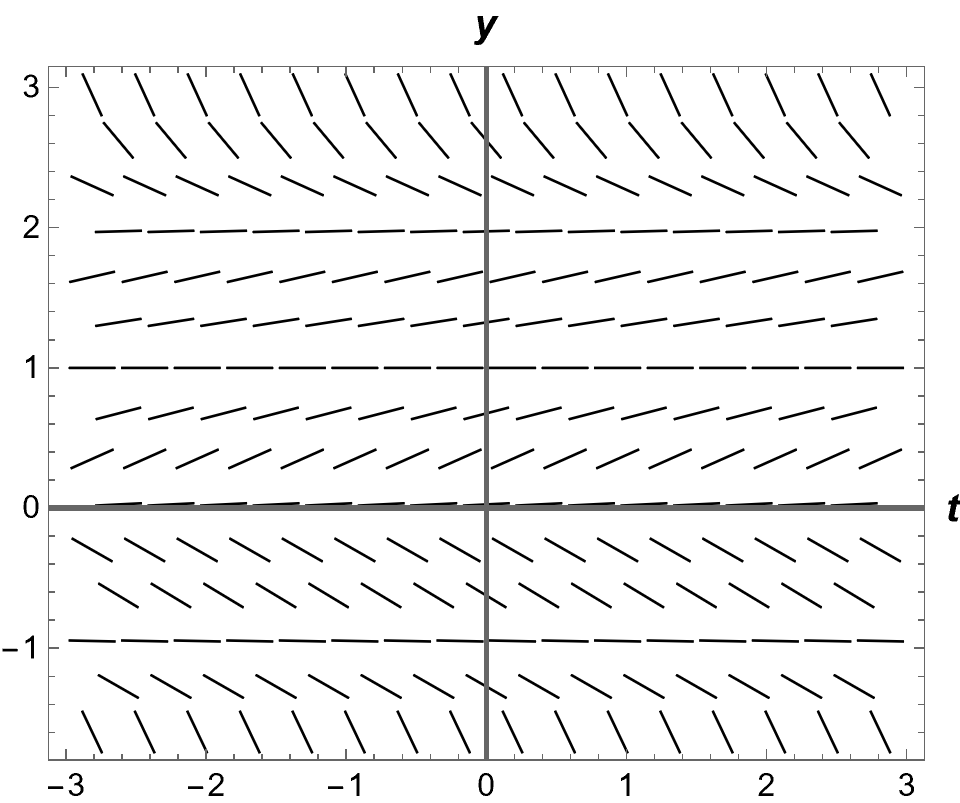
\includegraphics[scale=0.7,alt={A direction field.}]{ExemplarSevenDirectionField.png}
\caption{A direction field}
\end{figure}


\begin{enumerate}

\item Let's determine all the equilibrium solutions.

\vfill

\item Let's classify each equilibrium solution as asymptotically stable, semistable, or unstable.

\vfill

\newpage


\item Suppose $y(t)$ is a solution to $y^{\,\prime}=-\dfrac{(y^2-2y)(y^2-1)^2}{\sqrt{1+y^8}}$ satisfying that $y(0)=0.5$.  Let's determine $\displaystyle \lim_{t\rightarrow \infty} y(t)$.

\vfill

\item Let's determine the possible limits as $t\rightarrow \infty$ for non-constant solutions to \\$y^{\,\prime}=-\dfrac{(y^2-2y)(y^2-1)^2}{\sqrt{1+y^8}}$.

\vfill

\end{enumerate}

\newpage

 A \underline{second order autonomous equation} is one of the form $y^{\,\prime\prime}=f(y,y^{\,\prime})$.  
 
 Let's consider a second special case: $y^{\,\prime\prime}=f(y)$.

 \begin{enumerate}
    \item  By multiplying both sides by $y^{\,\prime}$ we get  $y^{\,\prime}y^{\,\prime\prime}=f(y)y^{\,\prime}$.  Then we can integrate both sides (with respect to the independent variable).  Let's determine what we get when we doe this, Using that $y^{\,\prime\prime} \mathrm{d}t=\mathrm{d}(y^{\,\prime})$ and $y^{\,\prime} \mathrm{d}t=\mathrm{d}y$.  The result is a separable differential equation.

    % (y^{\,\prime})^2 /2 = F(y)+C

    \vfill
    

    \item Let's  solve  the IVP $y^3y^{\,\prime\prime}=-1$, $y(1)=1$, $y^{\,\prime}(1)=-1$ using this method.


% y' y'' = -1/y^3 y'
% (y')^2 /2 = 1/(2y^2) +C
% (y')^2  = 1/y^2 +C.  y(1)=1 and y'(1)=-1 so (-1)^2=1/1^2+C implies C=0.
% (y')^2  = 1/y^2
% y' = - 1/y
% yy' = -1
% y^2 /2 = -t+C
% y^2  = C-2t
% y  = Sqrt[3-2t]
    
\vfill
\vfill
\vfill

     
 \end{enumerate}


\end{document}